\section*{Pendule à N maillons}

Dans cette partie, nous allons nous intéresser au pendule à $N$ maillons, dont la modélisation fait intervenir des équations différentielles.
\vskip 1mm ~

Nous avons commencé par modéliser le pendule à un unique maillon. 
Pour modéliser le pendule, nous avons besoin de deux données, l'angle $\theta$ et la vitesse angulaire $\omega$.
La relation entre la dérivée de $\theta$ et $\omega$, l'expression de la dérivée de $\omega$ en fonction de $\theta$ et le problème de Cauchy sont définis dans l'équation~\ref{eq:simple_pendulum}.

\begin{equation}
	\theta' = \omega \qquad \omega' = -\frac{g}{L}\sin(\theta) \quad
	\begin{cases}
		\theta' = \omega\\
		\omega' = -\frac{g}{L}\sin(\theta)
	\end{cases}
	\label{eq:simple_pendulum}
\end{equation}

Nous avons implémenté une fonction permettant de déterminer la fréquence d'oscillation du système (\verb|determine_frequency|) en fonction de l'angle initial $\theta$. Pour cela, nous résolvons 
le problème de Cauchy défini de l'équation~\ref{eq:simple_pendulum} avec $N=10000$ et $h = \frac{10}{N}$. Après résolution, nous avons la vitesse angulaire pour $t \in [0,10]$. Ensuite,
pour calculer la période $T$, nous cherchons le premier maximum local, puis nous cherchons le second maximum local. Enfin, nous calculons la fréquence $f = \frac{1}{T}$.

La figure~\ref{fig:frequency} illustre cette fréquence pour un pendule de longueur $l=1$ et de masse $m=1$. On remarque que la fréquence est, pour de petites valeurs de $\theta$, très proche de $\frac{1}{2\pi}\sqrt{\frac{g}{l}}$. On peut donc en déduire graphiquement que, pour de petites oscillations, la fréquence est égale à $\frac{1}{2\pi}\sqrt{\frac{g}{l}}$.

\begin{figure}[ht]
	\centering
	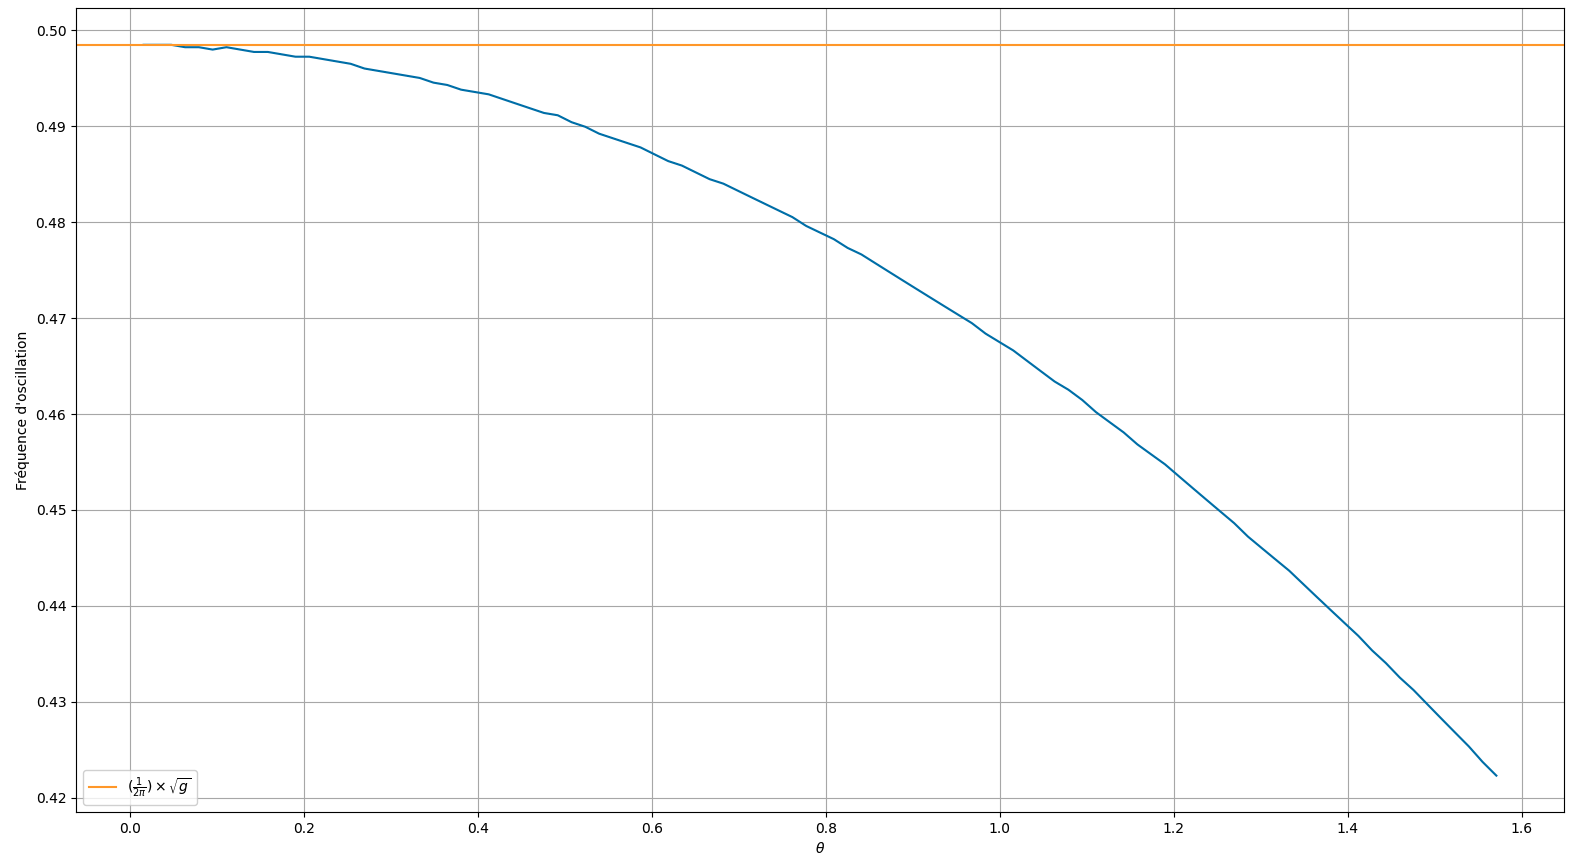
\includegraphics[width=0.6\textwidth]{img/frequency}
	\caption{Fréquence d'oscillation du pendule à un unique maillon en fonction de l'angle initial $\theta$}
	\label{fig:frequency}
\end{figure}

Ensuite, nous avons modélisé le pendule à deux maillons. Pour cela, nous nous sommes appuyés sur les équations usuelles\footnote{Source : \url{www.myphysicslab.com/dbl_pendulum.html}}.
\vskip 1mm ~

Le système à deux maillons est un système chaotique : le système dépend fortement des conditions initiales. La figure~\ref{fig:chaos}, représentant la trajectoire de l'extrémité du pendule à deux maillons en fonction du temps, illustre ce phénomène. Cette figure a été réalisée avec $50$ valeurs de $\theta$ réparties dans l'intervalle $[0,1]$. On posera alors, dans le cadre de notre modèle, $\theta_1 = \theta$ et $\theta_2 = -\theta$.

\begin{figure}[ht]
	\centering
	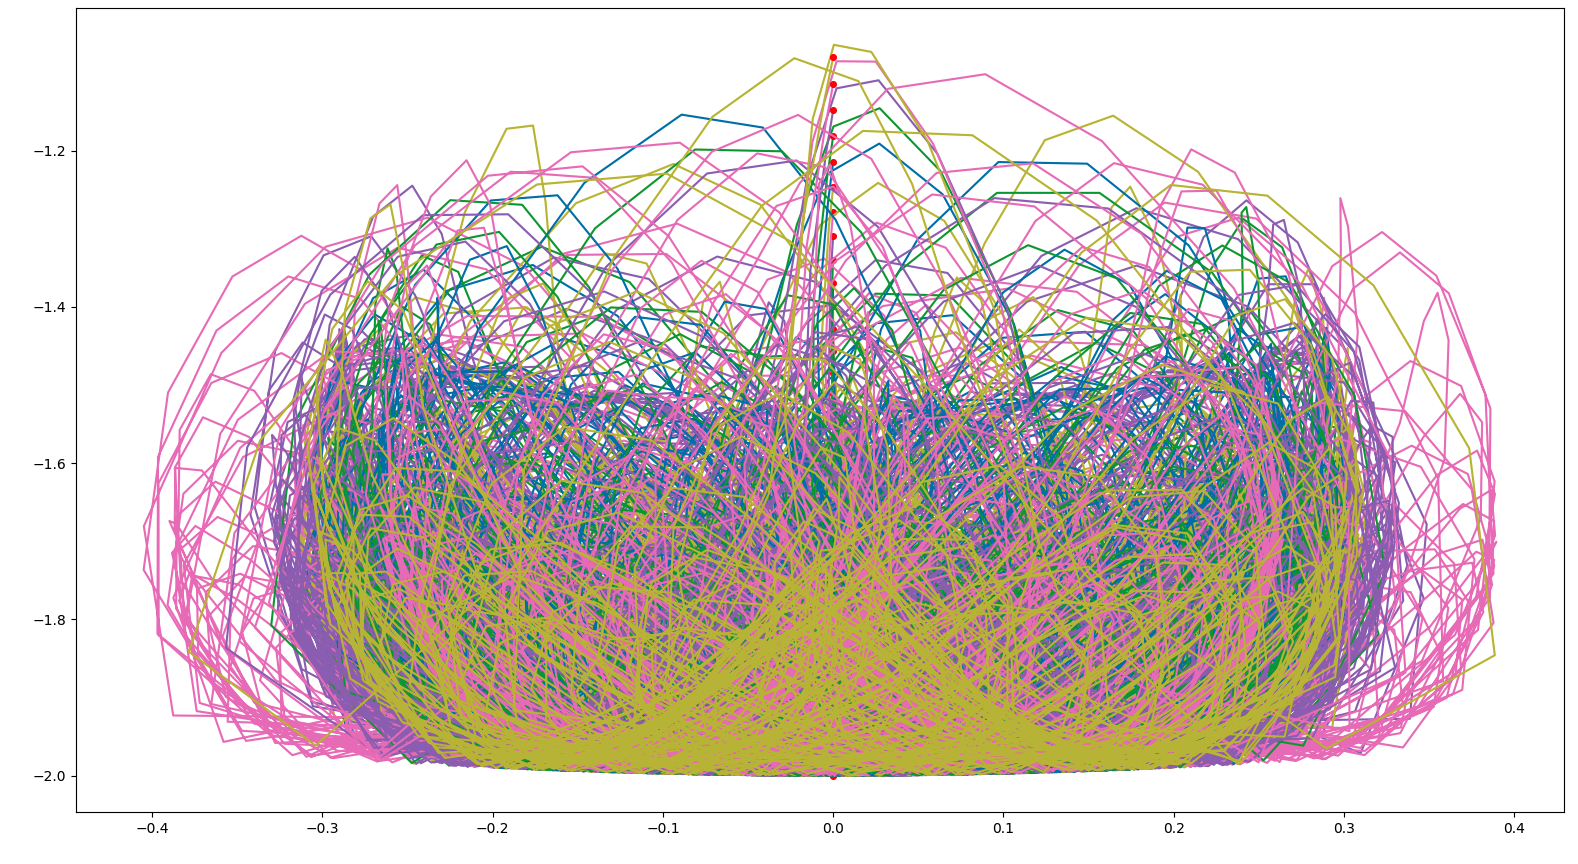
\includegraphics[width=0.6\textwidth]{img/chaos}
	\caption{Trajectoires d'un pendule à 2 maillons placé dans différentes conditions initiales}
	\label{fig:chaos}
\end{figure}

Enfin, nous avons déterminé numériquement le terme du premier retournement du pendule. Une carte représentant ce temps est représentée en figure~\ref{fig:flip_time}. Cette figure illustre bien la forte dépendance aux conditions initiales du système, chaque couleur\footnote{On retrouver la correspondances des couleurs ici : \url{https://en.wikipedia.org/wiki/Double\_pendulum\#Chaotic\_motion}} indiquant si l'un des pendules se retourne pour une période donnée.

\begin{figure}[H]
	\centering
	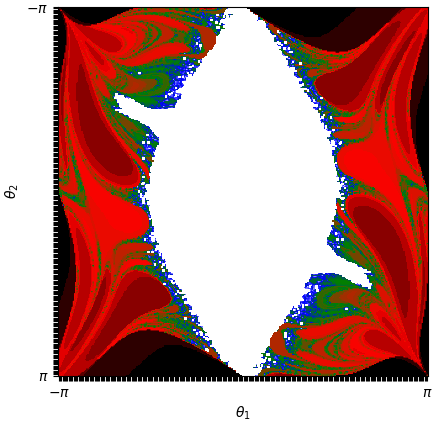
\includegraphics[width=0.60\textwidth]{img/flip_time_300x300}
	\caption{Temps de retournement du pendule en fonction des conditions initiales}
	\label{fig:flip_time}
\end{figure}